\documentclass[12pt]{article}
\usepackage[a4paper, total={5.5in, 9in}]{geometry}
\usepackage{amsmath}
\usepackage{amsfonts}
\usepackage{graphicx}
\usepackage{pgfplots}
\pgfplotsset{compat=1.18}
\usepackage{enumitem}

\title{College Algebra Worksheet 5.3}
\author{PCL Learning Center}
\date{}

\begin{document}
\maketitle

\section*{Problem Set 1\\Difficulty level: Normal}
\section*{Problem 1}
Find the $x$-intercepts and $y$-intercept of the following function.

\[ f(x) = (x - 1)(x + 1)(x + 2) \]

\section*{Problem 2}
Find the $x$-intercepts and $y$-intercept of the following function.

\[ f(x) = (x - 5)(x + 1)(3x + 6) \]

\section*{Problem 3}
Given that the polynomial $f(x)$ has degree 4, which of the following most accurately describes the number of turning points of $f(x)$?

\begin{enumerate}[label=(\Alph*)]
    \item The graph of $f(x)$ has at least 5 turning points.
    \item The graph of $f(x)$ has at least 4 turning points.
    \item The graph of $f(x)$ has at most 5 turning points.
    \item The graph of $f(x)$ has at most 3 turning points.
    \item The graph of $f(x)$ has at most 4 turning points.
    \item The graph of $f(x)$ has at least 3 turning points.
\end{enumerate}

\section*{Problem 4}
Given that the polynomial $f(x)$ has 9 turning points, which of the following most accurately describes the degree of $f(x)$?

\begin{enumerate}[label=\Alph*)]
    \item The degree of $f(x)$ is at most 10.
    \item The degree of $f(x)$ is at most 8.
    \item The degree of $f(x)$ is at least 10.
    \item The degree of $f(x)$ is at most 9.
    \item The degree of $f(x)$ is at least 9.
    \item The degree of $f(x)$ is at least 8.
\end{enumerate}

\section*{Problem 5}
Given the graph of the following degree 3 polynomial function, find all of the zeros and their multiplicities.

\begin{figure}[!ht]
    \centering
    \includegraphics[width=0.5\linewidth]{1.png}
\end{figure}

$x = \underline{\hspace{1cm}}$ with multiplicity $\underline{\hspace{1cm}}$, and $x = \underline{\hspace{1cm}}$ with multiplicity $\underline{\hspace{1cm}}$.

\section*{Problem 6}
Given the graph of the following degree 4 polynomial function, find all of the zeros and their multiplicities.

\begin{figure}[!ht]
    \centering
    \includegraphics[width=0.5\linewidth]{2.png}
\end{figure}

\newpage
\begin{enumerate}[label=\Alph*)]
    \item $x = -1$, with multiplicity 1, $x = 2$, with multiplicity 2, and $x = -3$, with multiplicity 1
    \item $x = 1$, with multiplicity 2, $x = 2$, with multiplicity 1, and $x = -3$, with multiplicity 1
    \item $x = -1$, with multiplicity 1, $x = 2$, with multiplicity 1, and $x = -3$, with multiplicity 2
    \item $x = -1$, with multiplicity 2, $x = 2$, with multiplicity 1, and $x = -3$, with multiplicity 1
    \item $x = 1$, with multiplicity 1, $x = 2$, with multiplicity 2, and $x = -3$, with multiplicity 1
    \item $x = -1$, with multiplicity 2, $x = -2$, with multiplicity 1, and $x = -3$, with multiplicity 1
\end{enumerate}

\section*{Problem 7}
Based on the graph of $f(x)$ shown below, which statement most accurately describes the degree of $f(x)$?

\begin{center}
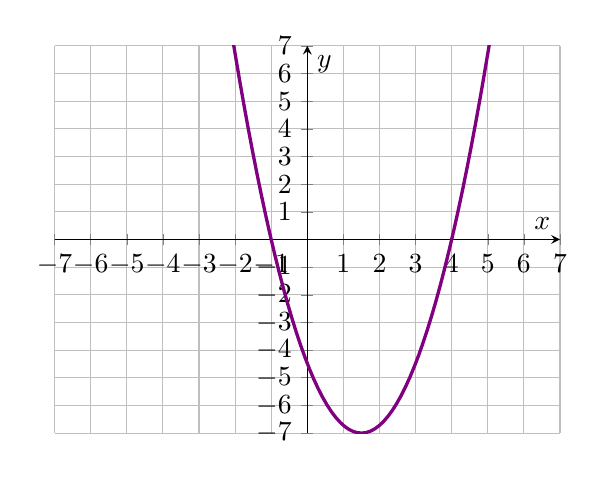
\begin{tikzpicture}
\begin{axis}[
    axis lines=middle,
    width=8cm,
    height=6.5cm,
    xmin=-7, xmax=7,
    ymin=-7, ymax=7,
    xtick={-7,...,7},
    ytick={-7,...,7},
    grid=both,
    xlabel=\(x\),
    ylabel=\(y\),
]
\addplot[domain=-6:6, samples=100, very thick, violet] {(28/25)*x^2-(84/25)*x-(112/25)};
\end{axis}
\end{tikzpicture}
\end{center}

\begin{enumerate}[label=\Alph*)]
    \item The polynomial has degree at least 2
    \item The polynomial has degree at most 3
    \item The polynomial has degree at most 1
    \item The polynomial has degree at most 2
    \item The polynomial has degree at least 3
    \item The polynomial has degree at least 1
\end{enumerate}

\section*{Problem 8}
Based on the graph of $f(x)$ shown below, what is the degree of $f(x)$?\\
\begin{figure}[!ht]
    \centering
    \includegraphics[width=0.5\linewidth]{3.png}
\end{figure}

The polynomial has degree at least \underline{\hspace{1cm}}.

\section*{Problem 9}
Write a polynomial, $P(x)$ in factored form given the following requirements.

\begin{itemize}
    \item Degree: 3
    \item $x$-intercepts at $(3,0)$, $(5,0)$ and $(1,0)$
    \item $y$-intercept at $(0,-15)$
\end{itemize}

\newpage
\section*{Problem 10}
Which is an equation with a degree of 3, $x$-intercepts located at $(7, 0)$ and $(-3, 0)$ and a $y$-intercept located at $(0, 84)$?

\begin{enumerate}[label=\Alph*)]
    \item $y = (x-3)(x-4)(x+7)$
    \item $y = (x+3)(x-4)(x-7)$
    \item $y = (x+3)(x+4)(x-7)$
    \item $y = (x-3)(x+4)(x+7)$
    \item $y = (x+3)(x-7)+84$
\end{enumerate}

\section*{Problem Set 2\\Difficulty level: Hard}
\section*{Problem 1}
For the following exercises, find the zeros and give the multiplicity of each.

    \begin{enumerate}
        \item[(a)] \((x+2)^3(x-3)^2\)
        \item[(b)] \(x^6-x^5-2x^4\)
        \item[(c)] \(4x^4(9x^4-12x^3+4x^2)\)
    \end{enumerate}

\newpage
\section*{Solutions to the Set 1}
\subsection*{Problem 1}
\(x\)-intercepts \(= (-2,0),(-1,0),(1,0)\)\\
\(y\)-intercepts \(= (0,-2)\)
\subsection*{Problem 2}
\(x\)-intercepts \(= (-2,0),(-1,0),(5,0)\)\\
\(y\)-intercepts \(= (0,-30)\)
\subsection*{Problem 3}
\begin{enumerate}
    \item[D)] The graph of $f(x)$ has at most 3 turning points.
\end{enumerate}
\subsection*{Problem 4}
\begin{enumerate}
    \item[C)] The degree of $f(x)$ is at least 10.
\end{enumerate}
\subsection*{Problem 5}
\(x=-3\) with multiplicity 1, and \(x=0\) with multiplicity 0.
\subsection*{Problem 6}
\begin{enumerate}
    \item[D)] $x = -1$, with multiplicity 2, $x = 2$, with multiplicity 1, and $x = -3$, with multiplicity 1
\end{enumerate}

\subsection*{Problem 7}
\begin{enumerate}
    \item[A)] The polynomial has degree at least 2
\end{enumerate}

\subsection*{Problem 8}
3

\subsection*{Problem 9}
\(P(x)=(x+1)(x-3)(x+5)\)
\subsection*{Problem 10}
\begin{enumerate}
    \item[B)] $y = (x+3)(x-4)(x-7)$
\end{enumerate}

\section*{Solutions to the Set 2}
\subsection*{Problem 1}
\begin{enumerate}
    \item[(a)] \(x=-2\) with multiplicity 3, and \(x=3\) with multiplicity 2.
    \item[(b)] \(x=-1\) with multiplicity 1, \(x=0\) with multiplicity 4, and \(x=2\) with multiplicity 1.
    \item[(c)] \(x=0\) with multiplicity 6, and \(x=\dfrac{2}{3}\) with multiplicity 2.
\end{enumerate}

\end{document}